\documentclass{article}

\usepackage[T1]{fontenc}    %Schriftart des Dokumentes
\usepackage[ngerman]{babel} %Dokumentensprache, hier Deutsch
\usepackage{amsmath, amssymb, stmaryrd} %mathematische Schriftzeichen
\usepackage{graphicx} %Einfügen von Grafiken
\usepackage{wrapfig}
\usepackage{bm}
\usepackage{subfig}
\usepackage{newclude}
\usepackage{pdfpages}
\usepackage{hyperref}
\hypersetup{
    colorlinks,
    citecolor=black,
    filecolor=black,
    linkcolor=black,
    urlcolor=black
}

\makeatletter
\newcommand\invisiblesection[1]{%
  \refstepcounter{section}%
  \addcontentsline{toc}{section}{\protect\numberline{\thesection}#1}%
  \sectionmark{#1}\phantom{}}
\makeatother

\setlength{\parindent}{0pt} %Einrückung von Absätzen auf null gesetzt
\setlength{\parskip}{10pt} %Abstand zischen Absätzen auf 10pt gesetzt

\title{Versuch 252: Aktivierung mit thermischen Neutronen}
\author{Matthias Kuntz}
\date{24.06.2024}

\renewcommand*\contentsname{Zusammenfassung}

\begin{document}

\maketitle

\tableofcontents

\newpage

%-------------------------EINLEITUNG-------------------------
\section{Einleitung}

In diesem Versuch soll die Aktivierung radioaktiver Quellen mit thermischen Neutronen untersucht werden. Dazu werden die Präparate $^{116}$In und $^{108}$Ag sowie $^{110}$Ag aktiviert und daraufhin die Zerfallsraten analysiert. Im Endeffekt sollen so die Halbwertszeiten der Präparate bestimmt werden.

\subsection{Physikalische Grundlagen}

Um eine radioaktive Quelle zu erzeugen werden stabile Isotope durch Kernreaktionen aktiviert. Besonders effektiv ist die Aktivierung mit thermischen Neutronen, da diese nicht die Coulomb-Barriere des Kerns überwinden müssen und viele Kerne einen großen Wirkungsquerschnitt für den Einfach langsamer Neutronen besitzen. Wird ein solches Neutron vom Kern eingefangen so entsteht ein Isotop mit einer um 1 erhöhten Massenzahl, welches radioaktiv sein kann, wie beispielsweise der aus dem stabilen Isotop $^{115}$In entstehende $\beta$-Strahler $^{116}$In. 

Es ist zu beachten, dass häufig auch sogenannte Isomere gebildet werden, also Nuklide mit gleicher Anzahl Neutronen und Protonen in einem unterschiedlichen Energiezustand zum primär gebildeten Isotop, die häufig auch verschiedene Halbwertszeiten besitzen.

Allgemein wird bei der Aktivierung eine gewisse Anzahl der Präparatskerne radioaktiv und somit ist die Rate der zerfallenden Kerne ebenso abhängig von der Anzahl der aktivierten Kerne. Die Aktivität $A(t)$ beschreibt die Zahl der Zerfälle pro Sekunde und ist gegeben als 

\begin{equation}
    A(t) = A_\infty (1 - e^{-\lambda t}),
\end{equation}

wobei Lambda die Zerfallskonstante darstellt, die mit der Halbwertszeit $T_{1/2}$ verbunden ist:

\begin{equation}
    T_{1/2} = \frac{\ln 2}{\lambda}.
    \label{eq:HWT}
\end{equation} 

Werden keine weiteren Kerne aktiviert so folgen die Zerfälle dem klassischen radioaktiven Zerfallsgesetz:

\begin{equation}
    A(t) = A_0 e^{- \lambda t}.
\end{equation}

Bei der Aktivierung von natürlichem Silber entstehen die beiden radioaktiven Silberisotope $^{108}$Ag und $^{110}$Ag. Da sich deren Halbwertszeiten unterscheiden kann durch die Länge der Aktivierungszeit das Verhältnis der beiden Isotope beeinflusst werden, siehe Abbildung \ref{fig:Verhältnis}

\begin{figure}[!h]
    \centering
    \resizebox{0.8\textwidth}{!}{
    \includegraphics{graphics/aktivierungsverhältnis.png}}
    \caption{Aktivierungsverhältnis bei unterschiedlicher Aktivierungszeit [Quelle: PAP2.2 Skript, S.70, Stand: 31.07.2024]}
    \label{fig:Verhältnis}
\end{figure}


\subsection{Versuchsaufbau}

Der Versuchsaufbau, zu sehen in Abbildung \ref{fig:aufbau}, besteht aus einem Geiger-Müller-Zählrohr, das auf einer Halterungsschiene angebracht ist, auf welcher ebenso das radioaktive Präparat in verstellbarem Abstand positioniert werden kann. Das Signal des Zählrohrs wird an das Betriebsgerät und über einen externen Zähler an einen Computer gesendet. Am Betriebsgerät können die Zählrohrspannung sowie die Messdauer eingestellt werden.

\begin{figure}[!b]
    \centering
    \resizebox{0.8\textwidth}{!}{
    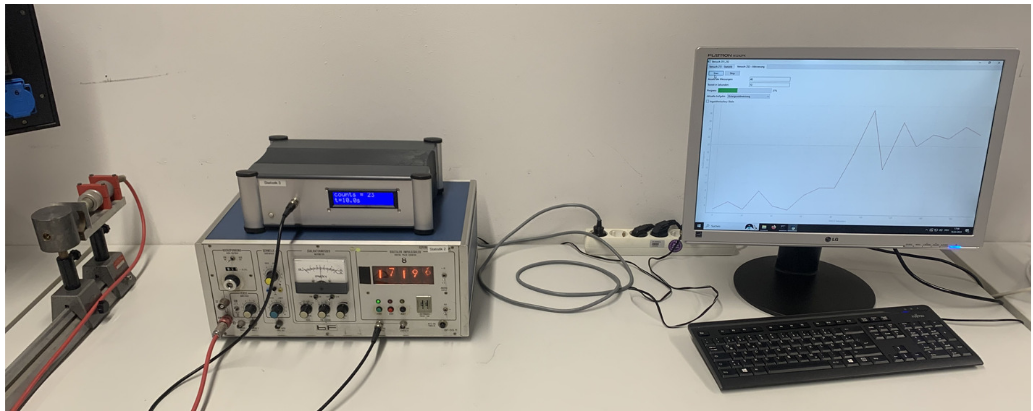
\includegraphics{graphics/aufbau.png}}
    \caption{Versuchsaufbau [Quelle: PAP2.2 Skript, S.69, Stand: 31.07.2024]}
    \label{fig:aufbau}
\end{figure}


\phantom{.}






%---------------VERSUCHSPROTOKOLL MIT MESSDATEN---------------
\newpage

\section{Versuchsprotokoll mit Messdaten}

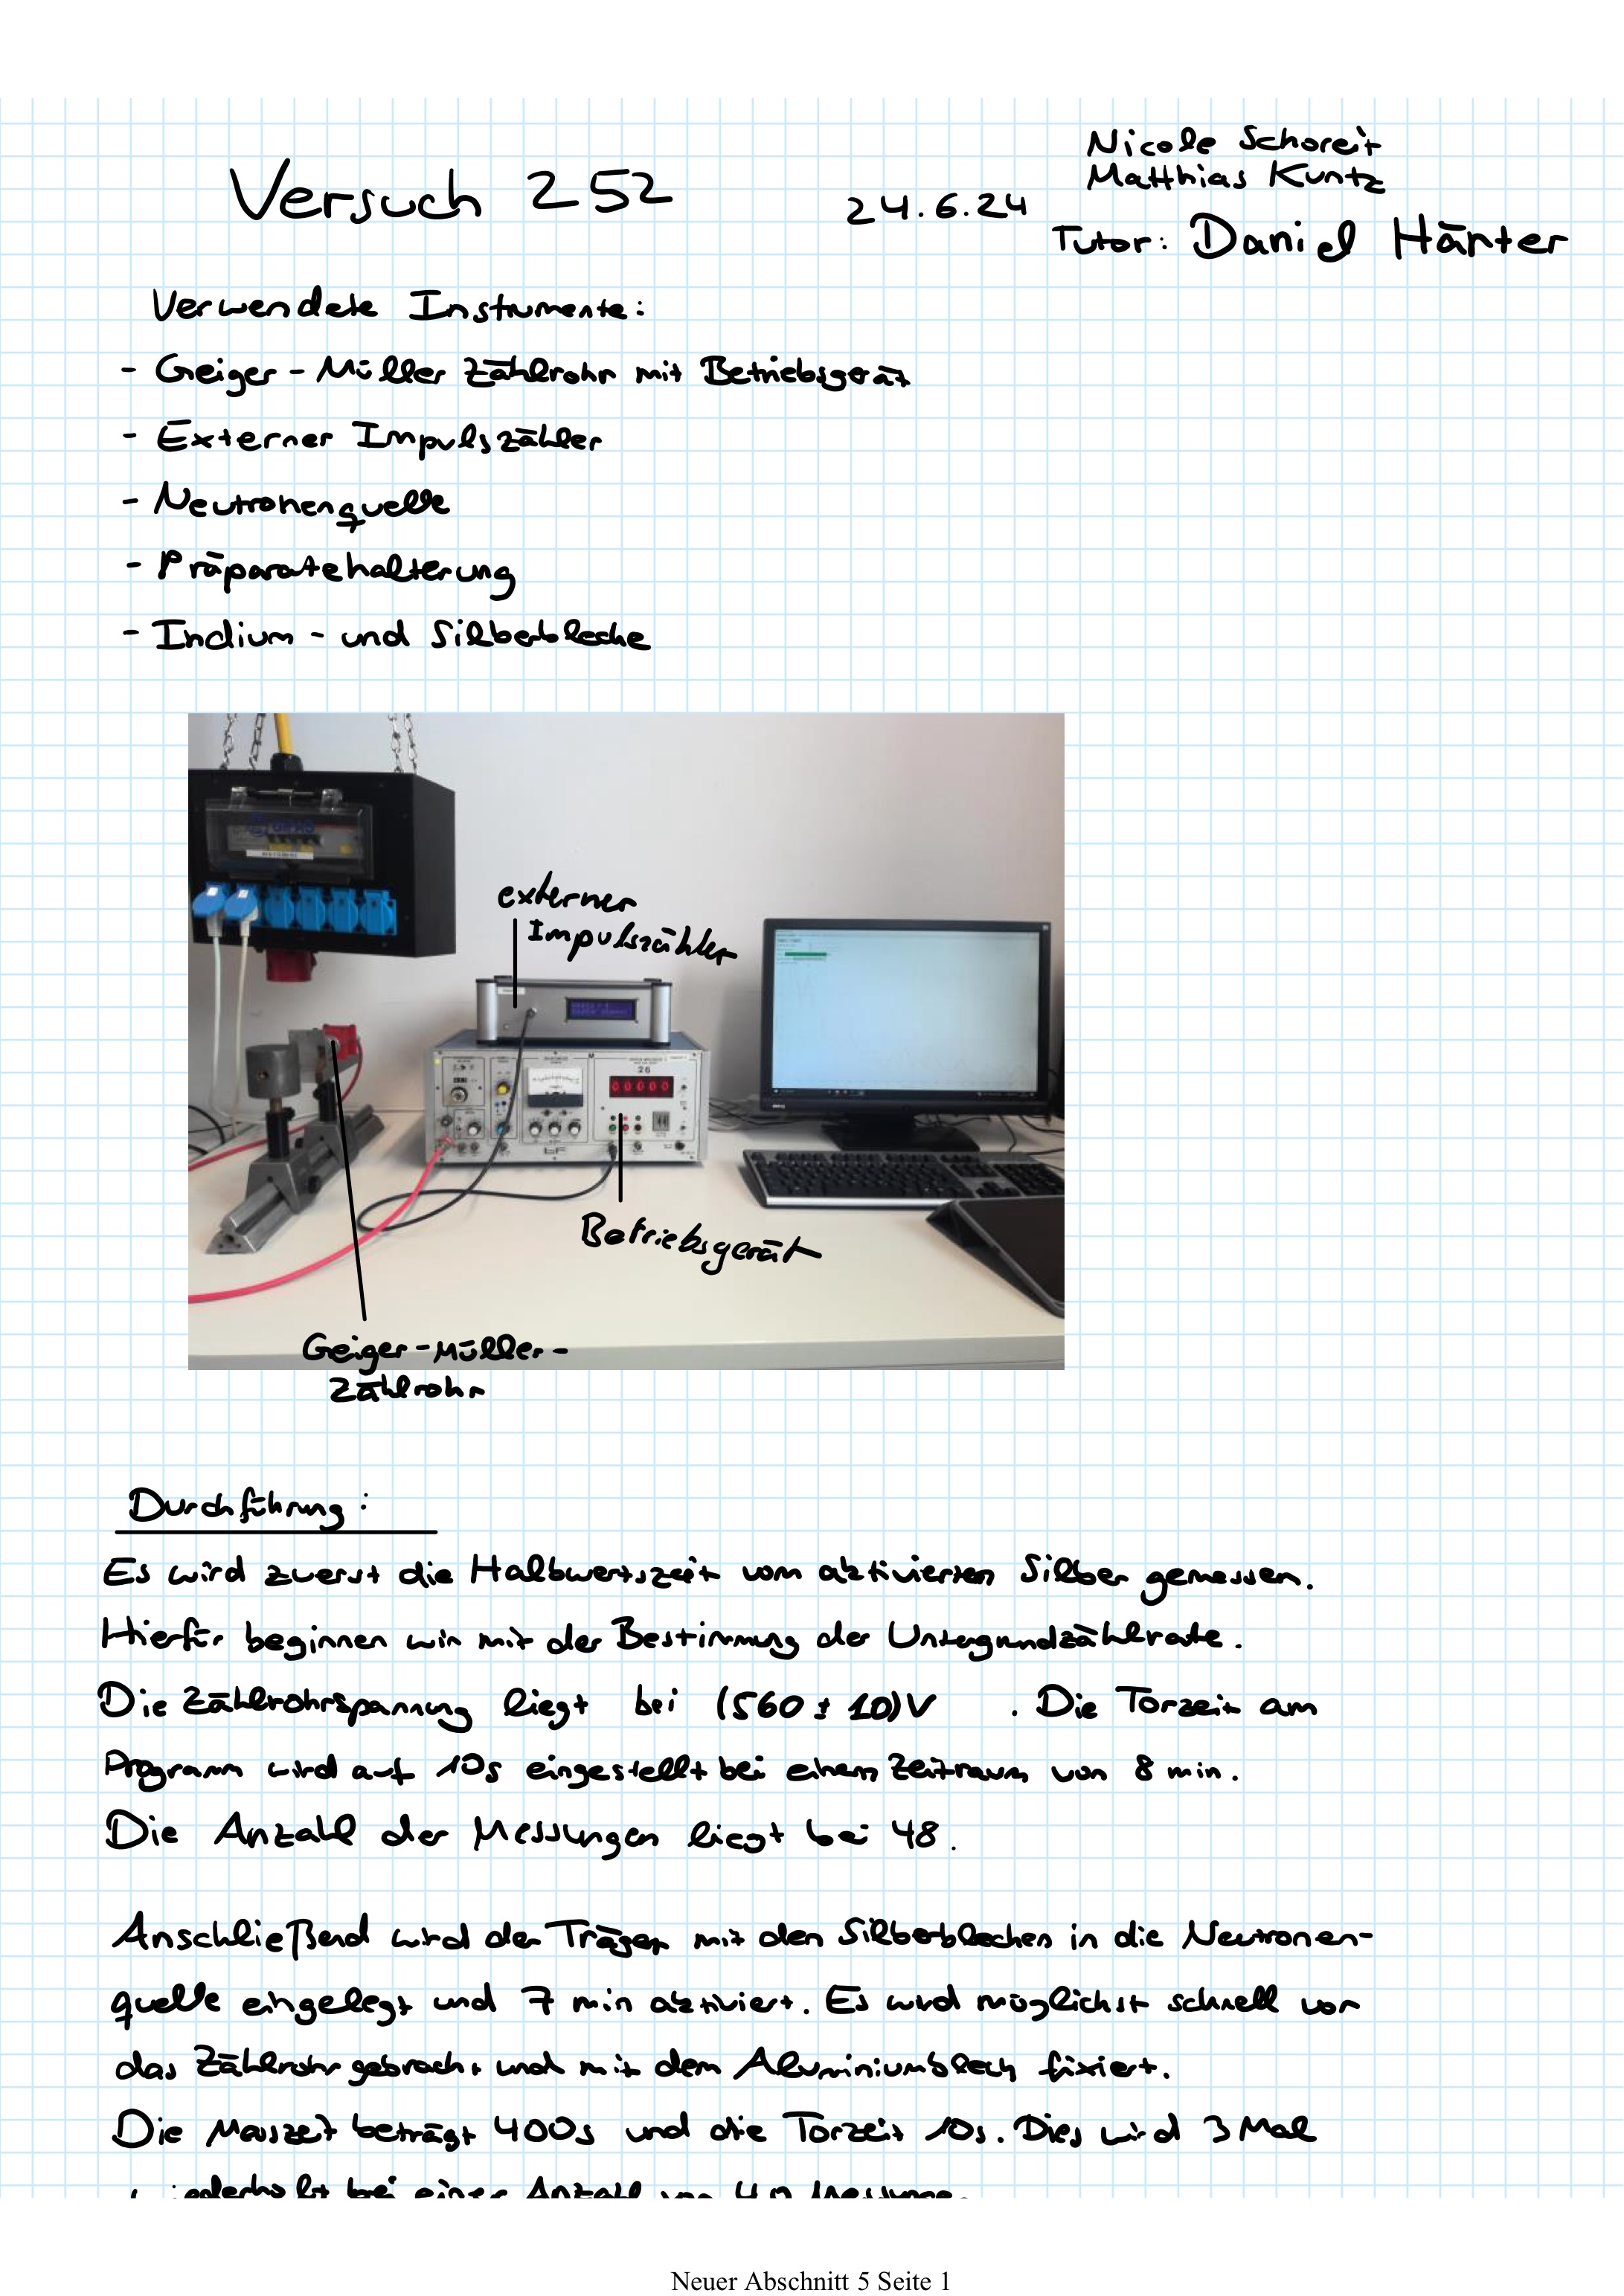
\includegraphics[width=\textwidth]{graphics/mess1.jpg}
\newpage
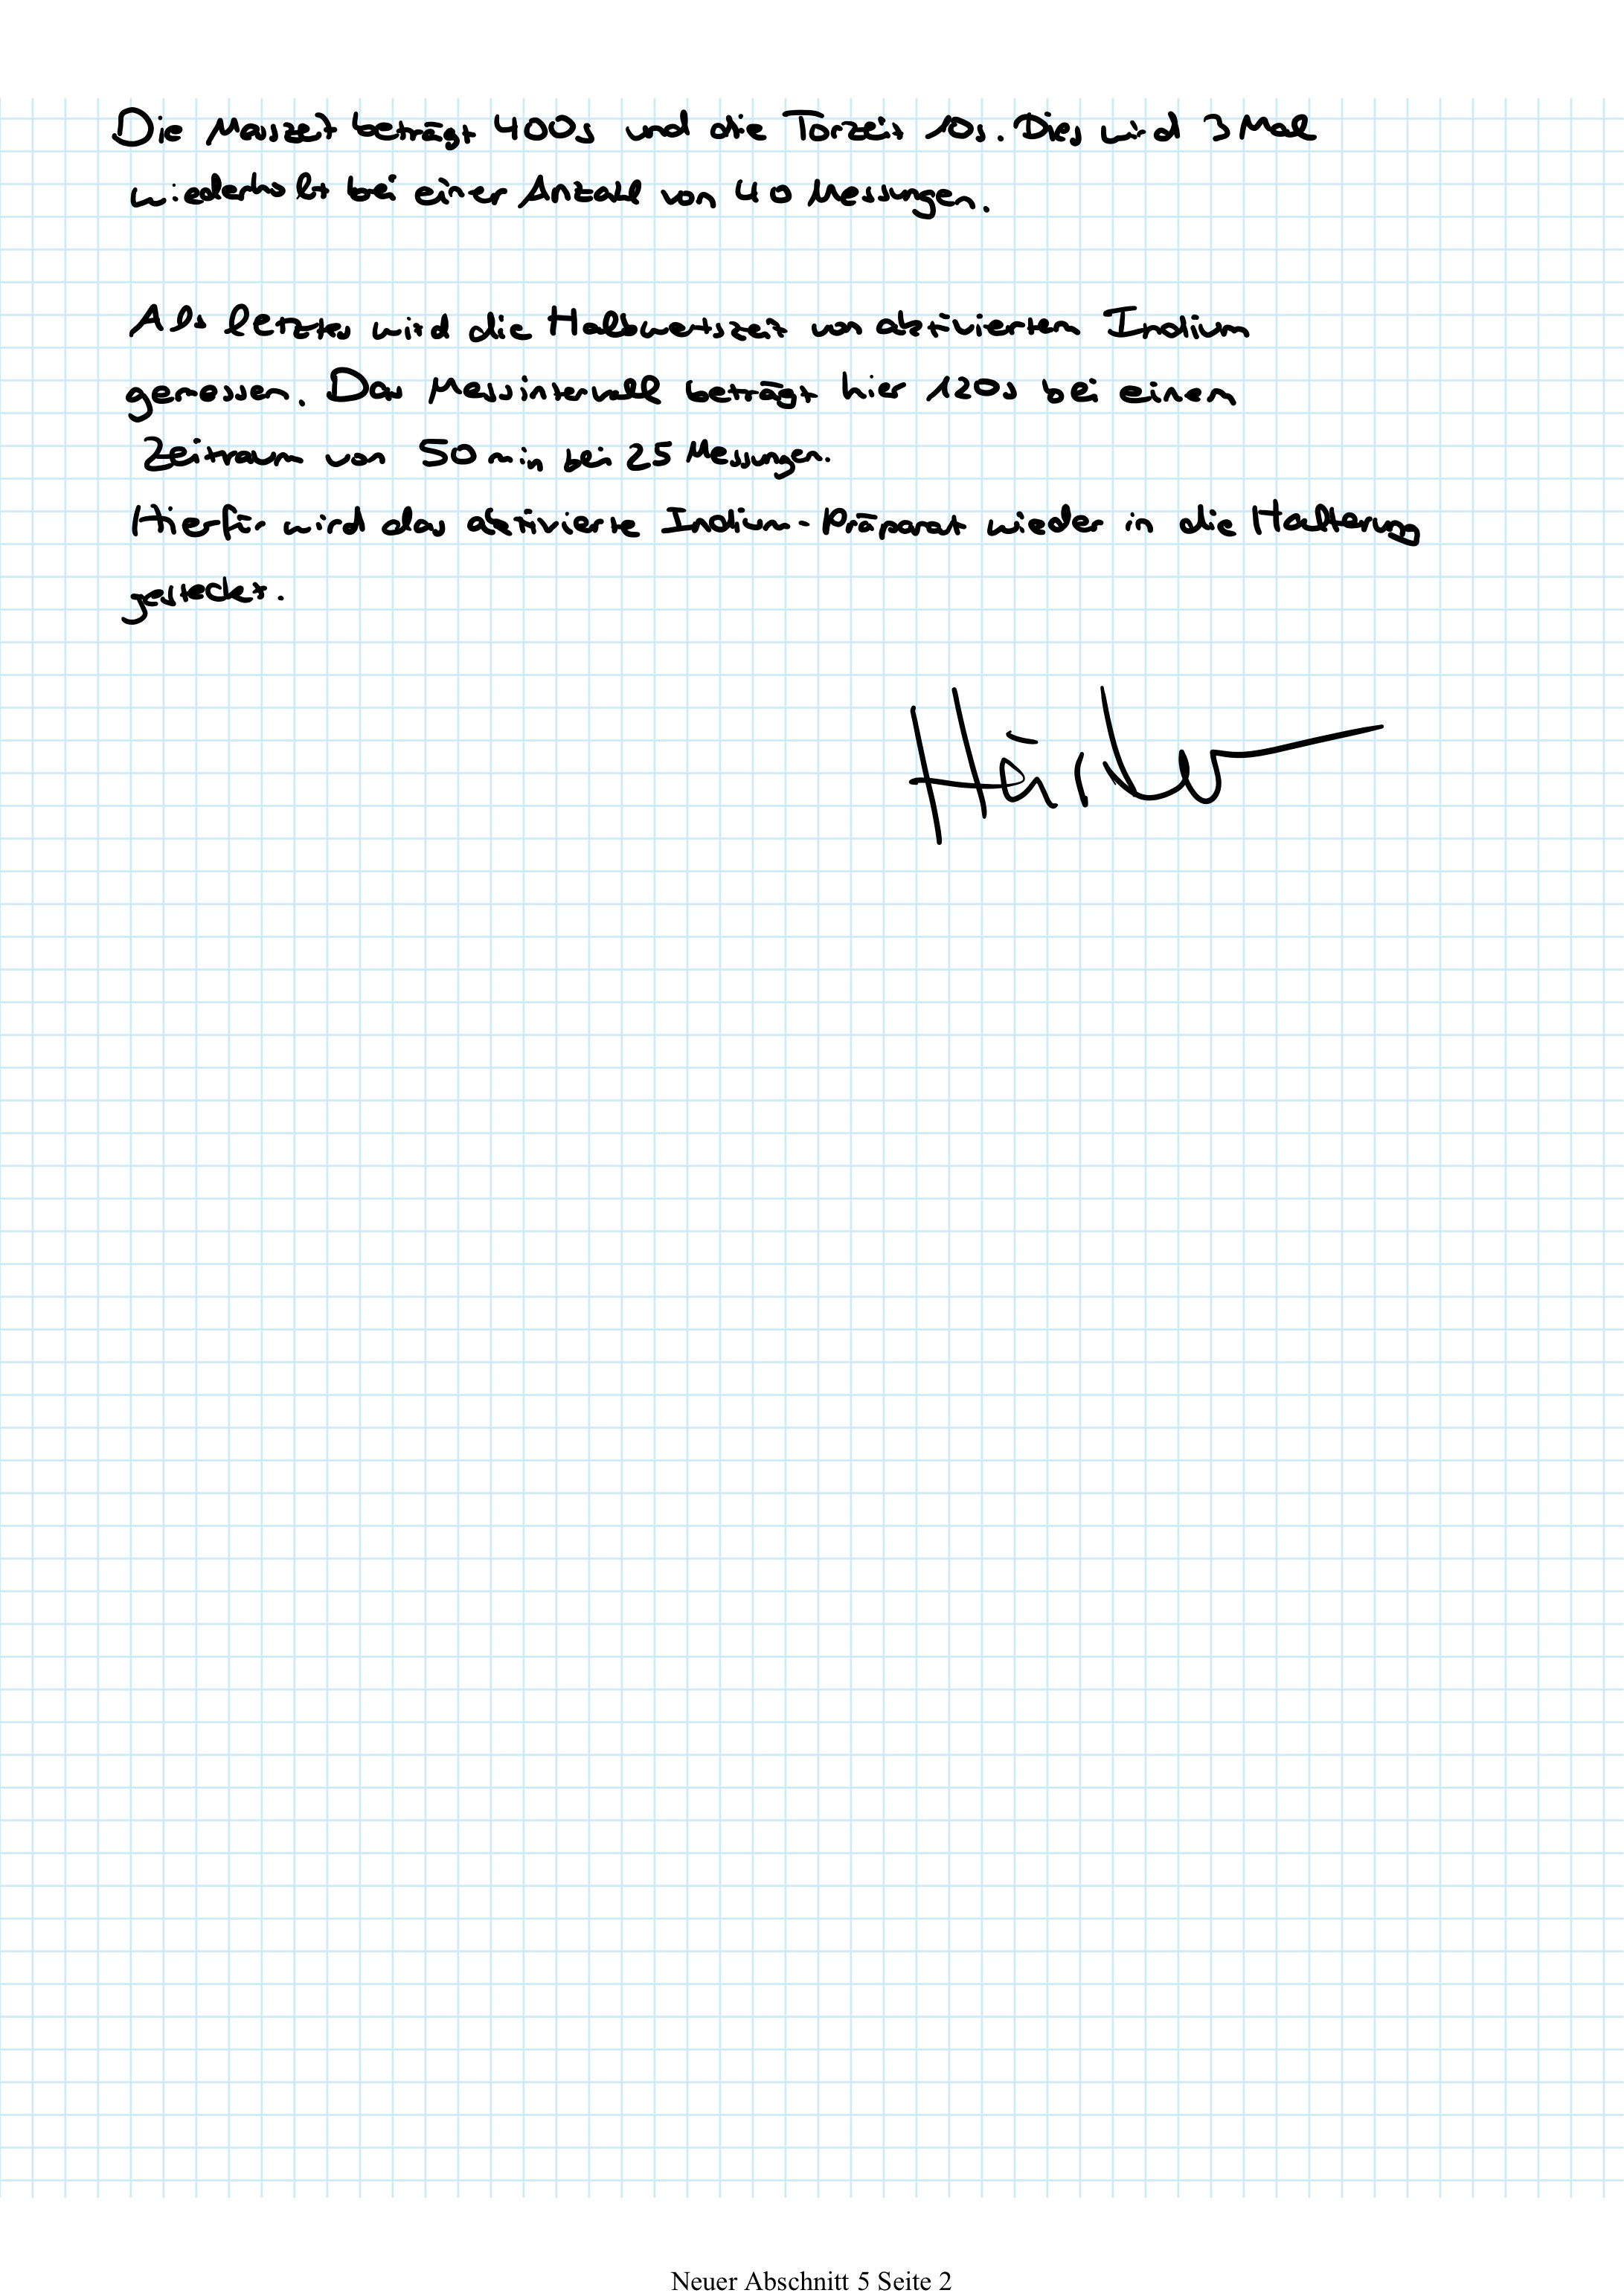
\includegraphics[width=\textwidth]{graphics/mess2.jpg}
\newpage





\clearpage
\newpage

\begin{table}[!p]

\begin{minipage}{0.47\textwidth}
\raggedleft
%\resizebox{\textwidth}{!}{
\begin{tabular}{cc}
\hline
$\bm{t}$ [s] & $\bm{N_{ug}}$ \\
\hline

        0 &      4 \\
        10 &      3 \\
        20 &      4 \\
        30 &      4 \\
        40 &      9 \\
        50 &      1 \\
        60 &      3 \\
        70 &      5 \\
        80 &      4 \\
        90 &      2 \\
        100 &      5 \\
        110 &      4 \\
        120 &      3 \\
        130 &      4 \\
        140 &      3 \\
        150 &      7 \\
        160 &      2 \\
        170 &      3 \\
        180 &      4 \\
        190 &      3 \\
        200 &      7 \\
        210 &      8 \\
        220 &      4 \\
        230 &      2 \\
        240 &      8 \\
        250 &      5 \\
        260 &      6 \\
        270 &      4 \\
        280 &      1 \\
        290 &      5 \\
        300 &      2 \\
        \vdots & \vdots \\
\hline
\end{tabular}%}

\end{minipage} \hfill
\begin{minipage}{0.47\textwidth}
\raggedright
%\resizebox{\textwidth}{!}{
\begin{tabular}{cc}
\hline
$\bm{t}$ [s] & $\bm{N_{ug}}$ \\
\hline
    
        \vdots & \vdots \\
        310 &      7 \\
        320 &      2 \\
        330 &      4 \\
        340 &      2 \\
        350 &      3 \\
        360 &      2 \\
        370 &      5 \\
        380 &      5 \\
        390 &      6 \\
        400 &      0 \\
        410 &      3 \\
        420 &      3 \\
        430 &      5 \\
        440 &      4 \\
        450 &      1 \\
        460 &      2 \\
        470 &      4 \\ 
        \phantom{.} & \\
        \phantom{.} & \\
        \phantom{.} & \\
        \phantom{.} & \\
        \phantom{.} & \\
        \phantom{.} & \\
        \phantom{.} & \\
        \phantom{.} & \\
        \phantom{.} & \\
        \phantom{.} & \\
        \phantom{.} & \\
        \phantom{.} & \\
        \phantom{.} & \\
        \phantom{.} & \\
\hline
\end{tabular}%}
\end{minipage} \hfill
\caption{Messwerte der Untergrundmessung}
\end{table}


\begin{table}[!p]
\begin{minipage}{0.5\textwidth}
\centering
\resizebox{\textwidth}{!}{
\begin{tabular}{ccccc}
\hline
$\bm{t}$ [s] & $\bm{N_1}$ & $\bm{N_2}$ & $\bm{N_3}$ & $\bm{N_4}$ \\
\hline
\phantom{\vdots} & \phantom{\vdots} & \phantom{\vdots} & \phantom{\vdots} & \phantom{\vdots} \\
            0 &   52 &   95 &  102 &   62 \\
            10 &   51 &   85 &   77 &   48 \\
            20 &   36 &   51 &   65 &   29 \\
            30 &   49 &   49 &   52 &   34 \\
            40 &   35 &   47 &   32 &   46 \\
            50 &   33 &   42 &   23 &   25 \\
            60 &   21 &   22 &   31 &   19 \\
            70 &   19 &   23 &   16 &   21 \\
            80 &   16 &   22 &   27 &   17 \\
            90 &   16 &   15 &   16 &   11 \\
            100 &   22 &    9 &   18 &   15 \\
            110 &   15 &   11 &   18 &    9 \\
            120 &   13 &   20 &   14 &   12 \\
            130 &   13 &   17 &   18 &   12 \\
            140 &   14 &   16 &   13 &    6 \\
            150 &    7 &   15 &   14 &   14 \\
            160 &    7 &   16 &    9 &    9 \\
            170 &   14 &    9 &    4 &    5 \\
            180 &   11 &   23 &   19 &    8 \\
            190 &   16 &    8 &    5 &    8 \\
            200 &    7 &    5 &    8 &   11 \\
            \vdots & \vdots & \vdots & \vdots & \vdots \\
\hline
\end{tabular}}
\end{minipage}
\begin{minipage}{0.5\textwidth}
\centering
\resizebox{\textwidth}{!}{
\begin{tabular}{ccccc}
\hline
$\bm{t}$ [s] & $\bm{N_1}$ & $\bm{N_2}$ & $\bm{N_3}$ & $\bm{N_4}$ \\
\hline
\vdots & \vdots & \vdots & \vdots & \vdots \\
    210 &   11 &   11 &   10 &    8 \\
    220 &    8 &    6 &    3 &    9 \\
    230 &   17 &   12 &   14 &    7 \\
    240 &   10 &    4 &   10 &    5 \\
    250 &    6 &    4 &    7 &   12 \\
    260 &    5 &    6 &    9 &    6 \\
    270 &    7 &    7 &    9 &    8 \\
    280 &   11 &    9 &   10 &    9 \\
    290 &    5 &    8 &   13 &    6 \\
    300 &    4 &    9 &    5 &    6 \\
    310 &    2 &    9 &    7 &    8 \\
    320 &    8 &    5 &    8 &    5 \\
    330 &    7 &    5 &    9 &    8 \\
    340 &    6 &    5 &    4 &    3 \\
    350 &    8 &    6 &    8 &    9 \\
    360 &    3 &    3 &    3 &    8 \\
    370 &    8 &    8 &    8 &    8 \\
    380 &    7 &   10 &    4 &    4 \\
    390 &    4 &    4 &    5 &    3 \\
    \phantom{.} & \phantom{.} & \phantom{.} & \phantom{.} & \phantom{.} \\
    \phantom{.} & \phantom{.} & \phantom{.} & \phantom{.} & \phantom{.} \\
    \phantom{\vdots} & \phantom{\vdots} & \phantom{\vdots} & \phantom{\vdots} & \phantom{\vdots} \\
\hline
\end{tabular}}
\end{minipage}
\caption{A1 - Silbermessungen}
\end{table}

\begin{table}[!p]
    \centering
    %\resizebox{\textwidth}{!}{
    \begin{tabular}{cc}
        \hline
        $\bm{t}$ [s] & $\bm{N_{ind}}$  \\ \hline
        0 &    765 \\
      120 &    693 \\
      240 &    694 \\
      360 &    691 \\
      480 &    623 \\
      600 &    609 \\
      720 &    606 \\
      840 &    569 \\
      960 &    591 \\
     1080 &    572 \\
     1200 &    609 \\
     1320 &    543 \\
     1440 &    525 \\
     1560 &    500 \\
     1680 &    460 \\
     1800 &    519 \\
     1920 &    491 \\
     2040 &    504 \\
     2160 &    489 \\
     2280 &    422 \\
     2400 &    430 \\
     2520 &    405 \\
     2640 &    413 \\
     2760 &    431 \\
     2880 &    385 \\ \hline
    \end{tabular}%}
    \caption{A2 - Indiummessung}
    \label{tab:A4-L1}
\end{table}


\clearpage
\newpage
%-------------------------AUSWERTUNG-------------------------
\section{Auswertung}

In dieser Evaluation werden alle Fehler, sofern keine spezifische Angabe gemacht wird, mithilfe der Gauss'schen Fehlerfortpflanzung berechnet. Dies bedeutet, dass ein Wert $F$, der mit der Formel $f(a_1, ..., a_n)$ berechnet wird, den Fehler $\Delta F$ annimmt:

\begin{equation}
    \Delta F = \sqrt{\sum_n \left( \frac{\partial f}{\partial a_n} \cdot \Delta a_n \right)^2}.
\end{equation}

Des Weiteren erfolgen Signifikanztests von zwei Werten $a$ und $a'$ über die folgende Formel:

\begin{equation}
    \sigma = \frac{|a-a'|}{\sqrt{(\Delta a)^2 + (\Delta a')^2}}.
\end{equation}

Die Auswertung sowie Berechnung erfolgen über das dem Dokument angehängte Python-Programm. Hierbei erfolgen Fits von Funktionen mithilfe der 'curve\_fit'-Funktion des 'SciPy'-Packages und Plots werden mit 'matplotlib' erstellt.

Die Güte eines Fits wird mit der $\chi^2$-Summe bewertet:

\begin{equation}
    \chi^2 = \sum_i^N \left( \frac{\textit{Funktionswert}_i - \textit{Messwert}_i}{\textit{Fehler}_i} \right)^2
\end{equation}

Auch verwendet wird $\chi^2_{red} = \chi^2 / f$, wobei der Freiheitsgrad $f$ die Anzahl der Messwerte minus die Anzahl der Fitparameter ist. Der auf die Freiheitsgrade normierte Wert soll bei einem guten Fit ungefähr 1 sein.


\newpage

\subsection{Zerfall der Silberisotope}

Wir beginnen, indem wir aus den Messdaten der Untergrundmessung den Mittelwert der Messrate bestimmen. Der Fehler ergibt sich hierbei einfach aus der Standardabweichung gemäß

\begin{equation}
    \sigma_{std} = \sqrt{\frac{1}{N} \sum_{i=1}^N (\overline{x} - x_i)^2}.
\end{equation}

Beide werden noch mit vier multipliziert, da wir die vier Messreihen der Silbermessungen addieren werden. Somit erhalten wir den vierfachen Mittelwert des Untergrunds:

\begin{equation}
    \overline{n}_{bkg} = (15,6 \pm 1,1) \text{counts/10s}.
\end{equation}

Nun importieren wir die Daten der vier Silbermessungen und addieren die Raten der vier Messungen aufeinander. Der Fehler ergibt sich statistisch aus $\sqrt{N}$. Wir stellen die resultierenden Raten als Funktion der Zeit dar und fitten die folgende doppelte Zerfallsfunktion:

\begin{equation}
    y = \alpha_1 e^{-\lambda_1 t} + \alpha_2 e^{-\lambda_2 t} + n_{bkg}.
\end{equation}

Somit erhalten wir einmal die Fitparameter für $^{108}$Ag und einmal für $^{110}$Ag. Wir wiederholen diesen Schritt für drei Werte von $n_{bkg}$. Einmal nutzen wir einfach den Mittelwert $\overline{n}_{bkg}$. Daraufhin addieren und subtrahieren wir jeweils einmal den Fehler des Mittelwerts, ergo wir verwenden $\overline{n}_{bkg} + 1\sigma$ und $\overline{n}_{bkg} - 1\sigma$. Somit erhalten wir insgesamt drei Plots, dargestellt in den Abbildungen \ref{fig:A1-SmUG} - \ref{fig:A1-SmUG-1} und drei Sätze an Fit-Parametern, welche in Tabelle \ref{tab:A1-Fits} eingetragen sind. 

\phantom{.}

\begin{table}[!h]
    \centering
    %\resizebox{\textwidth}{!}{
    \begin{tabular}{c|ccc}
        \hline
        $\bm{n_{bkg}}$ & $\bm{\overline{n}_{bkg}}$ & $\bm{\overline{n}_{bkg} + 1\sigma}$ & $\bm{\overline{n}_{bkg} - 1\sigma}$ \\ \hline
        $\bm{\alpha_1}$ & 273 $\pm$ 21 & 270 $\pm$ 22 & 276 $\pm$ 20 \\
        $\bm{\alpha_2}$ & 67 $\pm$ 20 & 69 $\pm$ 22 & 65 $\pm$ 18 \\
        $\bm{\lambda_1}$ [1/s] & 0,030 $\pm$ 0,004 & 0,030 $\pm$ 0,005 & 0,029 $\pm$ 0,004 \\
        $\bm{\lambda_2}$ [1/s] & 0,0059 $\pm$ 0,0012 & 0,0064 $\pm$ 0,0013 & 0,0055 $\pm$ 0,0011 \\ \hline
        $\bm{\chi^2}$ & 52,47 & 52,69 & 52,31  \\
        $\bm{\chi^2_{red}}$ & 1,46 & 1,46 & 1,45  \\
        \textbf{Wsk.} [\%] & 4,0 & 4,0 & 4,0  \\ \hline
    \end{tabular}%}
    \caption{A1 - Silbermessung - Fitparameter und Fitbewertung}
    \label{tab:A1-Fits}
\end{table}

\phantom{.}

Wir machen nun die folgenden vereinfachenden Definitionen: $\lambda_i = \lambda_i(\overline{n}_{bkg})$ und $\lambda_i^\pm = \lambda_i(\overline{n}_{bkg} \pm 1\sigma)$. Somit haben wir die Werte unserer Zeitkonstanten gegeben durch die $\lambda_i$ und können die Fehler folgendermaßen berechnen:

\begin{equation}
    \begin{split}
        \xi_i^\pm &= |\lambda_i - \lambda_i^\pm|, \\
        \Xi_i &= \frac{1}{2} (\xi_i^+ + \xi_i^-), \\ \\
        \Rightarrow \Delta \lambda_i &= \sqrt{(\Delta \lambda_i')^2 + \Xi_i^2}.
    \end{split}
\end{equation}

Hierbei bezeichnet $\Delta \lambda_i'$ den ursprünglichen Fehler der Fitparameter, so wie er in Tabelle \ref{tab:A1-Fits} steht. Wir erhalten somit die folgenden beiden Werte für die Zerfallskonstanten:

\begin{equation}
    \begin{split}
        {\lambda_1} &= {(0,030 \pm 0,004)} \text{1/s}, \\
        {\lambda_2} &= {(0,0059 \pm 0,0013)} \text{1/s}.
    \end{split}
\end{equation}

Und somit die folgenden Werte für die Halbwertszeiten gemäß Gleichung \ref{eq:HWT}:

\begin{equation}
    \begin{split}
        \bm{T_1} &= \bm{(23 \pm 3)} \textbf{s}, \\
        \bm{T_2} &= \bm{(117 \pm 25)} \textbf{s}.
    \end{split}
\end{equation}

Somit lässt sich identifizieren, dass der Index 1 das Präparat $^{110}$Ag und der Index 2 $^{108}$Ag bezeichnet. Die jeweiligen Literaturwerte sind gegeben als $T_{1,lit} = 24.6$s und $T_{2,lit} = 2,41 \text{min} = 144,6$s, wodurch wir Abweichungen von $0,40\sigma$ für $^{110}$Ag und $1,08\sigma$ für $^{108}$Ag erhalten, was beides insignifikante Abweichungen sind. 


\begin{figure}[!h]
    \centering
    \resizebox{0.9\textwidth}{!}{
    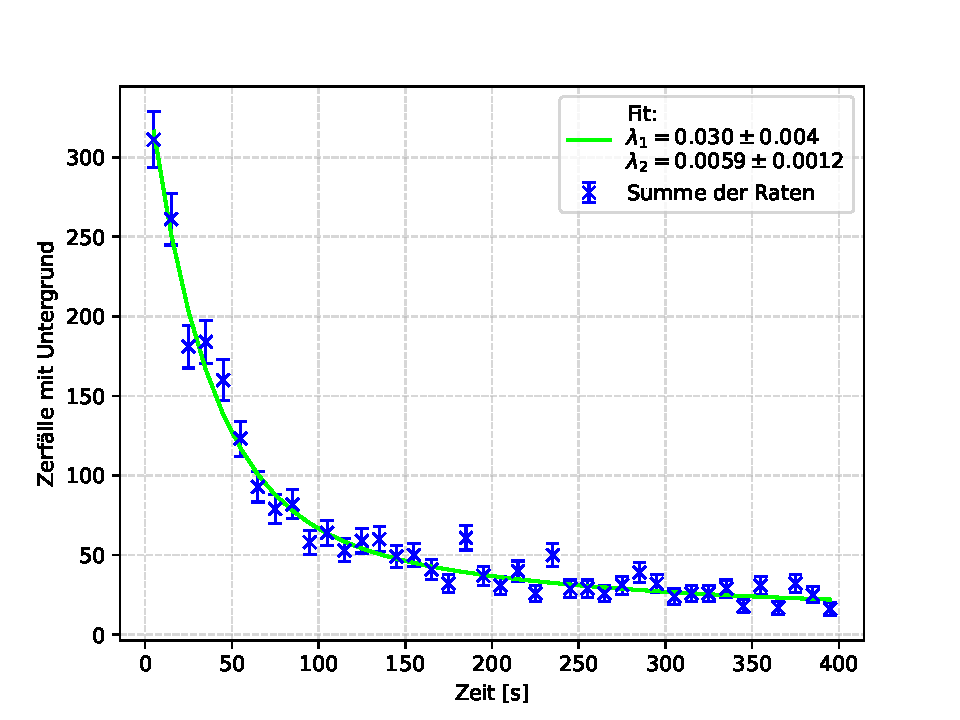
\includegraphics{plots/Silber_mit_UG.pdf}}
    \caption{A1 - Silberzerfall mit $\overline{n}_{bkg}$}
    \label{fig:A1-SmUG}
\end{figure}

\begin{figure}[!h]
    \centering
    \resizebox{0.9\textwidth}{!}{
    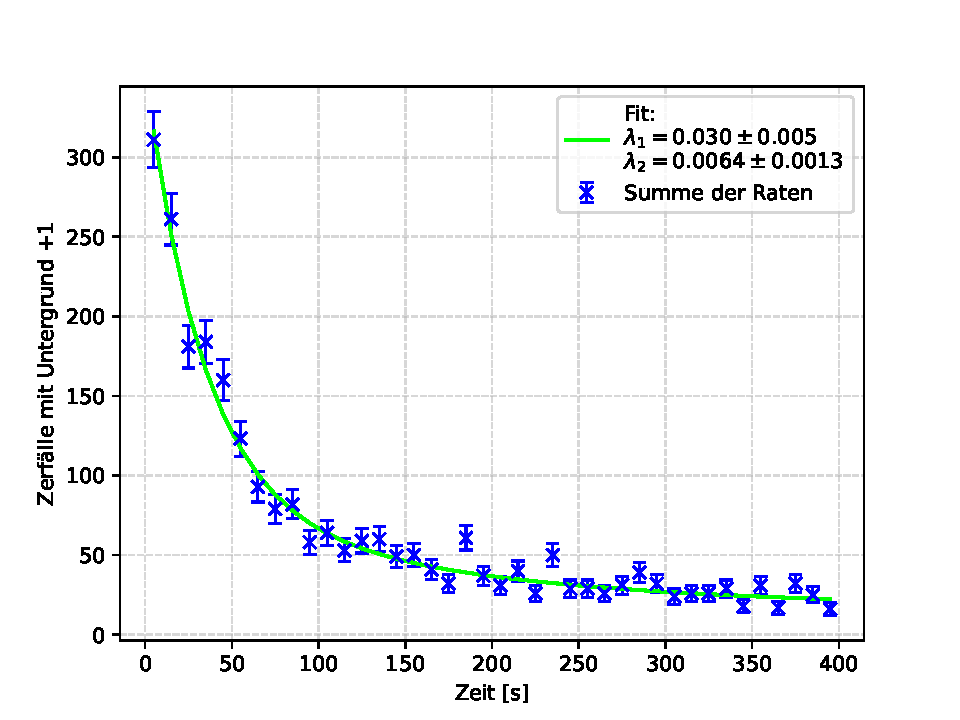
\includegraphics{plots/Silber_mit_UG+1.pdf}}
    \caption{A1 - Silberzerfall mit $\overline{n}_{bkg} + 1\sigma$}
    \label{fig:A1-SmUG+1}
\end{figure}

\begin{figure}[!h]
    \centering
    \resizebox{0.9\textwidth}{!}{
    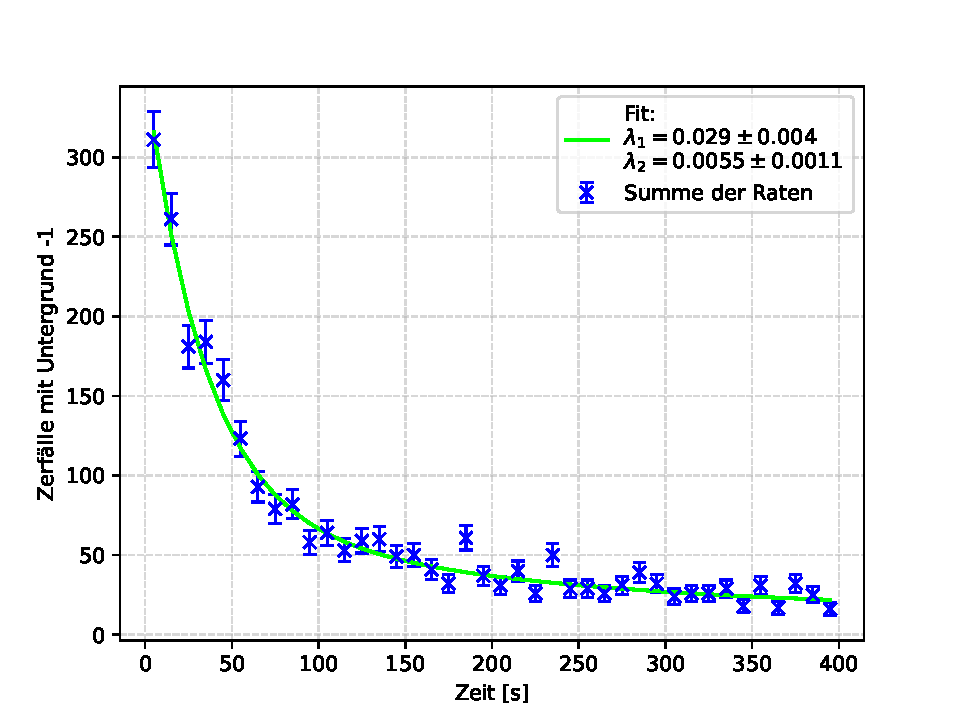
\includegraphics{plots/Silber_mit_UG-1.pdf}}
    \caption{A1 - Silberzerfall mit $\overline{n}_{bkg} - 1\sigma$}
    \label{fig:A1-SmUG-1}
\end{figure}


\clearpage
\newpage

\subsection{Zerfall vom Indiumisotop}

Zunächst passen wir den Untergrundwert an die Messdaten der Indium-Messung an. Da wir hier wieder nur eine Messung haben, dafür aber 12-Mal so lange jeweils gemessen haben, müssen wir den Wert von $\overline{n}_{bkg}$ mit dem Faktor 3 multiplizieren.

Nun machen wir genau die gleichen Schritte wie zuvor bei Silber. Da bei Indium allerdings nach kurzer Zeit keine nennenswerten Isomere vorhanden sind wie bei Silber, reicht es eine einfache Exponentialfunktion anzufitten und den ersten stark abweichenden Messwert zu vernachlässigen:

\begin{equation}
    y = \alpha e^{-\lambda t} + n_{bkg}.
\end{equation}

Wir machen wieder unsere drei Fits und erhalten die Diagramme in Abbildung \ref{fig:A2-ImUG} - \ref{fig:A2-ImUG-1} und die Fitparameter in Tabelle \ref{tab:A2-Fits}.

\phantom{.}

\begin{table}[!h]
    \centering
    %\resizebox{\textwidth}{!}{
    \begin{tabular}{c|ccc}
        \hline
        $\bm{n_{bkg}}$ & $\bm{\overline{n}_{bkg}}$ & $\bm{\overline{n}_{bkg} + 1\sigma}$ & $\bm{\overline{n}_{bkg} - 1\sigma}$ \\ \hline
        $\bm{\alpha}$ & 675 $\pm$ 13 & 672 $\pm$ 13 & 678 $\pm$ 13 \\
        $\bm{\lambda}$ [$10^{-5}$ 1/s] & 22,3 $\pm$ 1,2 & 22,5 $\pm$ 1,2 & 22,2 $\pm$ 1,2 \\ \hline
        $\bm{\chi^2}$ & 24,81 & 24,81 & 24,80  \\
        $\bm{\chi^2_{red}}$ & 1,13 & 1,13 & 1,13  \\
        \textbf{Wsk.} [\%] & 31,0 & 31,0 & 31,0  \\ \hline
    \end{tabular}%}
    \caption{A2 - Indiummessung - Fitparameter und Fitbewertung}
    \label{tab:A2-Fits}
\end{table}

\phantom{.}

Wir berechnen analog zu eben die Zerfallskonstante sowie damit die Halbwertszeit und erhalten:

\begin{equation}
    \lambda = (22,3 \pm 1,2) \cdot 10^{-5} 1/\text{s}
\end{equation}

\begin{equation}
    \bm{T = (3,10 \pm 0,17) \cdot 10^3} \textbf{s}
\end{equation}

Der Literaturwert für $^{116}$In ist gegeben als $T = 54 \text{min} = 3240$s womit wir eine Abweichung von $0,83\sigma$ erhalten, was insignifikant ist.

\begin{figure}[!h]
    \centering
    \resizebox{0.9\textwidth}{!}{
    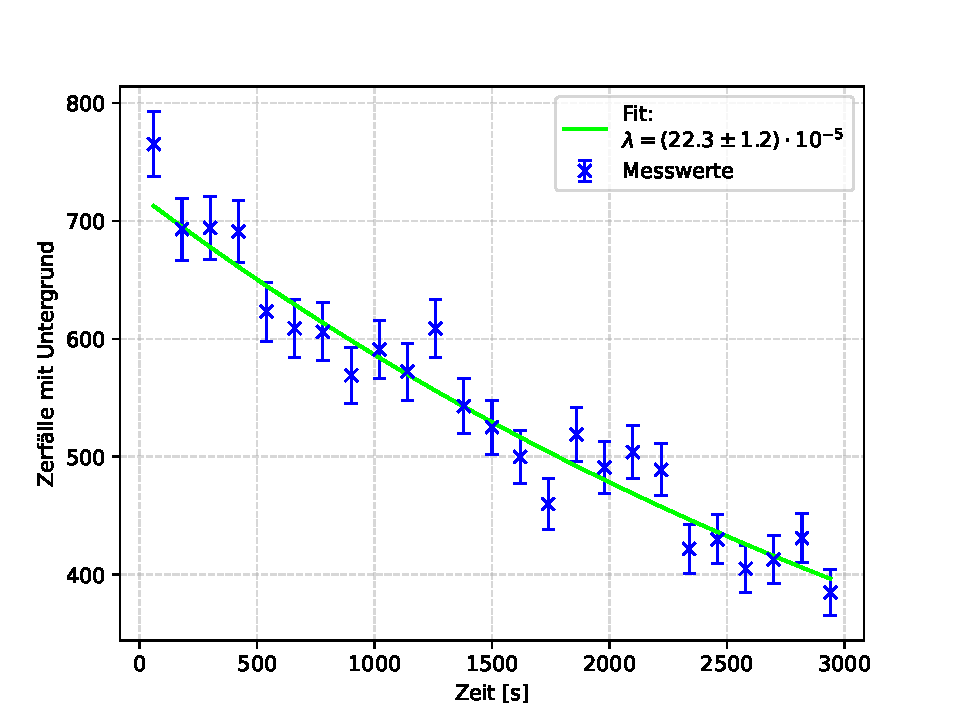
\includegraphics{plots/Indium_mit_UG.pdf}}
    \caption{A2 - Indiumzerfall mit $\overline{n}_{bkg}$}
    \label{fig:A2-ImUG}
\end{figure}

\begin{figure}[!h]
    \centering
    \resizebox{0.9\textwidth}{!}{
    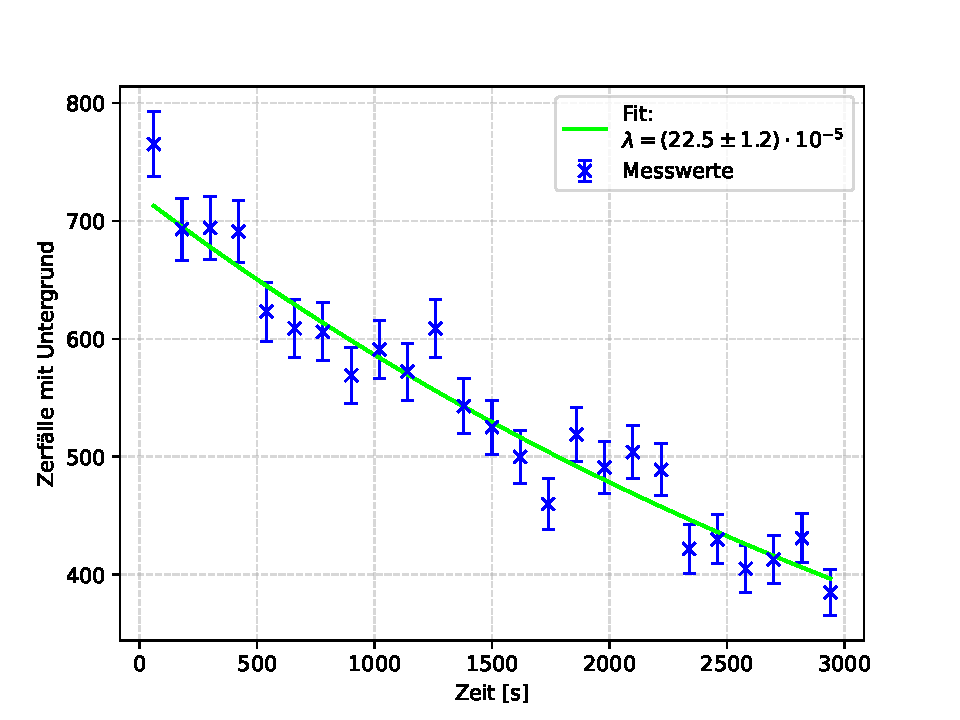
\includegraphics{plots/Indium_mit_UG+1.pdf}}
    \caption{A2 - Indiumzerfall mit $\overline{n}_{bkg} + 1\sigma$}
    \label{fig:A2-ImUG+1}
\end{figure}

\begin{figure}[!h]
    \centering
    \resizebox{0.9\textwidth}{!}{
    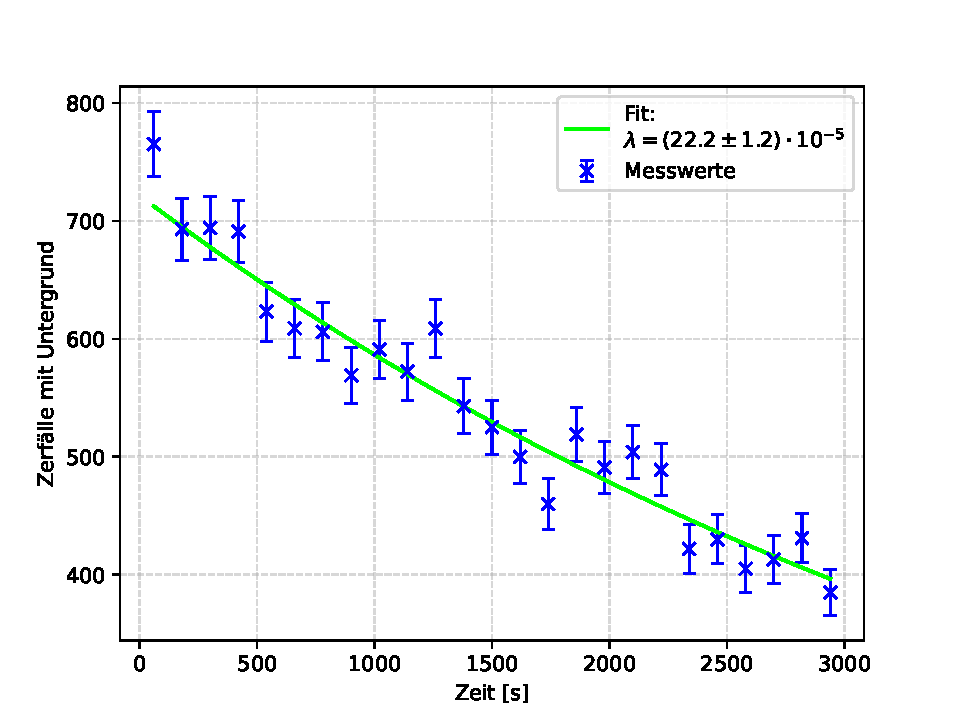
\includegraphics{plots/Indium_mit_UG-1.pdf}}
    \caption{A2 - Indiumzerfall mit $\overline{n}_{bkg} - 1\sigma$}
    \label{fig:A2-ImUG-1}
\end{figure}



\clearpage
\newpage
%---------------PRÄSENTATION DER ENDERGEBNISSE---------------
\section{Zusammenfassung der Endergebnisse}

In diesem Versuch wurde der Zerfall von den Präparaten $^{116}$In und $^{108}$Ag sowie $^{110}$Ag nach der Aktivierung mit thermischen Neutronen analysiert. Durch Messung der abnehmenden Zerfallsrate nach der Aktivierung konnten die Halbwertszeiten für die drei Präparate bestimmt werden:

\begin{equation}
    \begin{split}
        T_{^{108}Ag} &= (117 \pm 25) \text{s} \\ 
        T_{^{110}Ag} &= (23 \pm 3) \text{s} \\ 
        T_{^{116}In} &= (3,10 \pm 0,17) \cdot 10^{3} \text{s} \\ 
    \end{split}
\end{equation}

Alle drei Halbwertszeiten lagen hierbei innerhalb insignifikanter Abweichungen von gegebenen Literaturwerten. 


%---------------ZUSAMMENFASSUNG UND DISKUSSION---------------
\section{Diskussion}

In diesem Versuch wurden durchweg positive Ergebnisse erzieht. Die drei berechneten Halbwertszeiten liegen alle innerhalb insignifikanter Abweichungen. Als Kritikpunkt an den Werten lässt sich nur nennen, das bei der Halbwertszeit von $^{108}$Ag der Fehler etwa 20\% des Werts beträgt und somit leicht erhöht ist. Die anderen Werte liegen mit Fehlern von ca. 13 bzw. 5 Prozent allerdings komplett innerhalb akzeptabler Umgebungen. 

Des Weiteren lässt sich noch nennen, dass die gemessenen Werte teils stark um den erwarteten Exponentialverlauf schwankten, was an den teilweise leicht erhöhten $\chi^2_{red}$-Werten und den damit verbundenen Fitwahrscheinlichkeiten erkennbar ist. Jedoch halten sich diese Schwankungen insgesamt in Grenzen und treten nicht über die bei einem statistischen Versuch erwarteten Abweichungen hinaus. 

Somit lässt sich insgesamt sagen, dass bei diesem Versuch aussagekräftige mit der Theorie übereinstimmende Ergebnisse erzielt wurden und somit eine interessante und lehrreiche Einführung in die Thematik der radioaktiven Aktivierung erfolgen konnte. 

 
\newpage
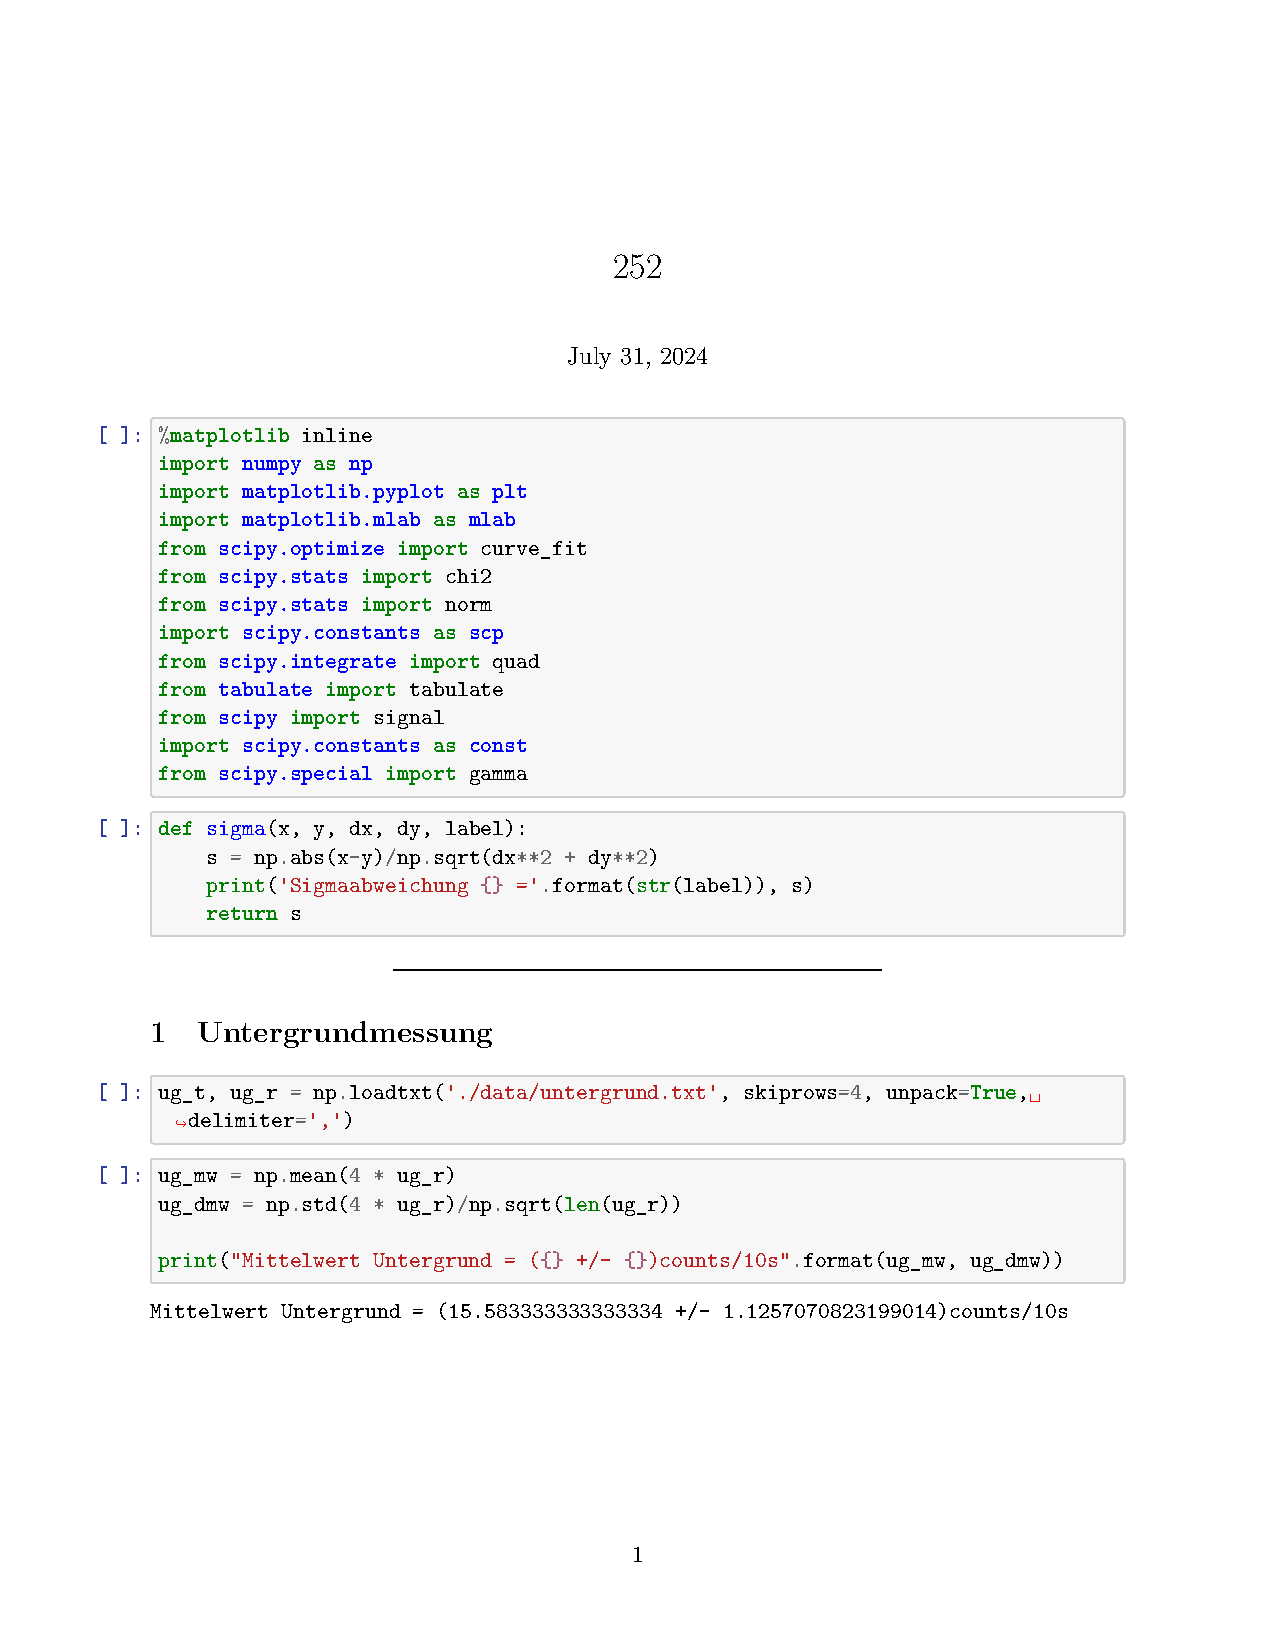
\includepdf[pagecommand=\invisiblesection{Python-Code},scale=0.8,pages=1]{./252.pdf}
\includepdf[pagecommand={},scale=0.8,pages=2-last]{./252.pdf}

\end{document}

